\documentclass[xcolor=dvipsnames,table]{beamer}

\usepackage{latexsym}
\usepackage[utf8]{inputenc}
\usepackage[portuguese]{babel}
\usepackage{amssymb}
\usepackage{amsmath}
\usepackage{stmaryrd}
\usepackage{fancybox}
\usepackage{datetime}
\usepackage[T1]{fontenc}
\usepackage{graphicx}
\usepackage{graphics}
\usepackage{url}
\usepackage{algorithmic}
\usepackage{algorithm}
\usepackage{acronym}
\usepackage{array}

\newtheorem{definicao}{Definio}
\newcommand{\tab}{\hspace*{2em}}

\mode<presentation>
{
  \definecolor{colortexto}{RGB}{0,0,0}
 
  \setbeamertemplate{background canvas}[vertical shading][ bottom=white!10,top=white!10]
  \setbeamercolor{normal text}{fg=colortexto} 

  \usetheme{Warsaw}
}

\title{EAD - Assignment 1} 

\author{
  Hélder Vieira \\ Miguel Tavares
  } 
 \institute{
  Estatística e Análise de Dados \\ MDS}
\date{\textbf{22 de junho de 2021} }



\begin{document}

	\begin{frame}
		\titlepage
	\end{frame}

%	\AtBeginSection{
%		\begin{frame}{Sumário}%[allowframebreaks]{Sumário}
%   		\tableofcontents[currentsection]
%    		%\tableofcontents[currentsection, hideothersubsections]
%		\end{frame}
%	}

	\begin{frame}{Índice}
		\tableofcontents
		%\tableofcontents[hideallsubsections]
	\end{frame}
	
	\section{Análise dos Dados}
	\subsection{Introdução}
	
	\begin{frame}{Introdução}
	    \begin{block}{World Happiness Report 2019}
	        \begin{itemize}
				\item 156 países
				\item 9 variáveis
				\begin{itemize}
				    \item \textit{Overall rank} (categ.)
				    \item \textit{Country or region} (categ.)
				    \item \textit{Score} (num.)
				    \item \textit{GDP per capita} (num.)
				    \item \textit{Social support} (num.)
				    \item \textit{Healthy life expectancy} (num.)
				    \item \textit{Freedom to make life choices} (num.)
				    \item \textit{Generosity} (num.)
				    \item \textit{Perceptions of Corruption} (num.)
				\end{itemize}
			\end{itemize}
		\end{block}
	\end{frame}
	
	\begin{frame}{Introdução}
	    Primeira abordagem:
	        \begin{itemize}
				\item Remoção da variável \textit{Overall rank};
				\item Agrupamento dos países por continente;
				\item Todas as variáveis resultantes de questionários (excepto \textit{GDP per capita} e \textit{Healthy life expectancy}).
			\end{itemize}
	\end{frame}
	
	\begin{frame}{Introdução}
		\begin{center}
    	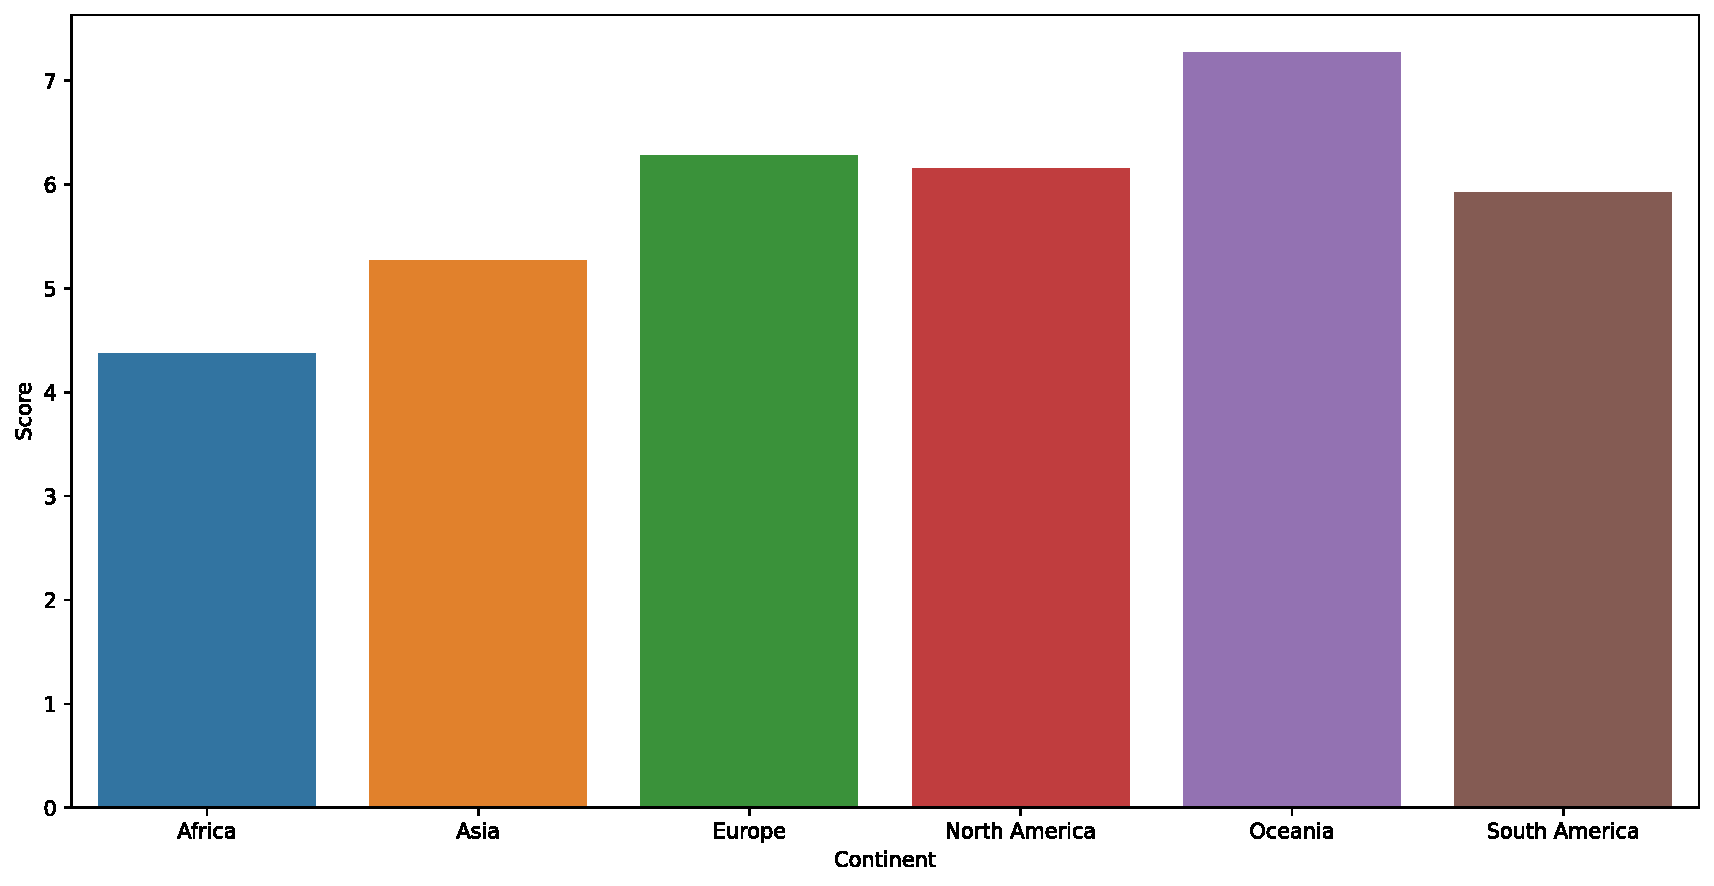
\includegraphics[height=.65\textheight]{score_continents.pdf}
  		\end{center}
	\end{frame}
	
	\begin{frame}{Introdução}
		\begin{center}
    	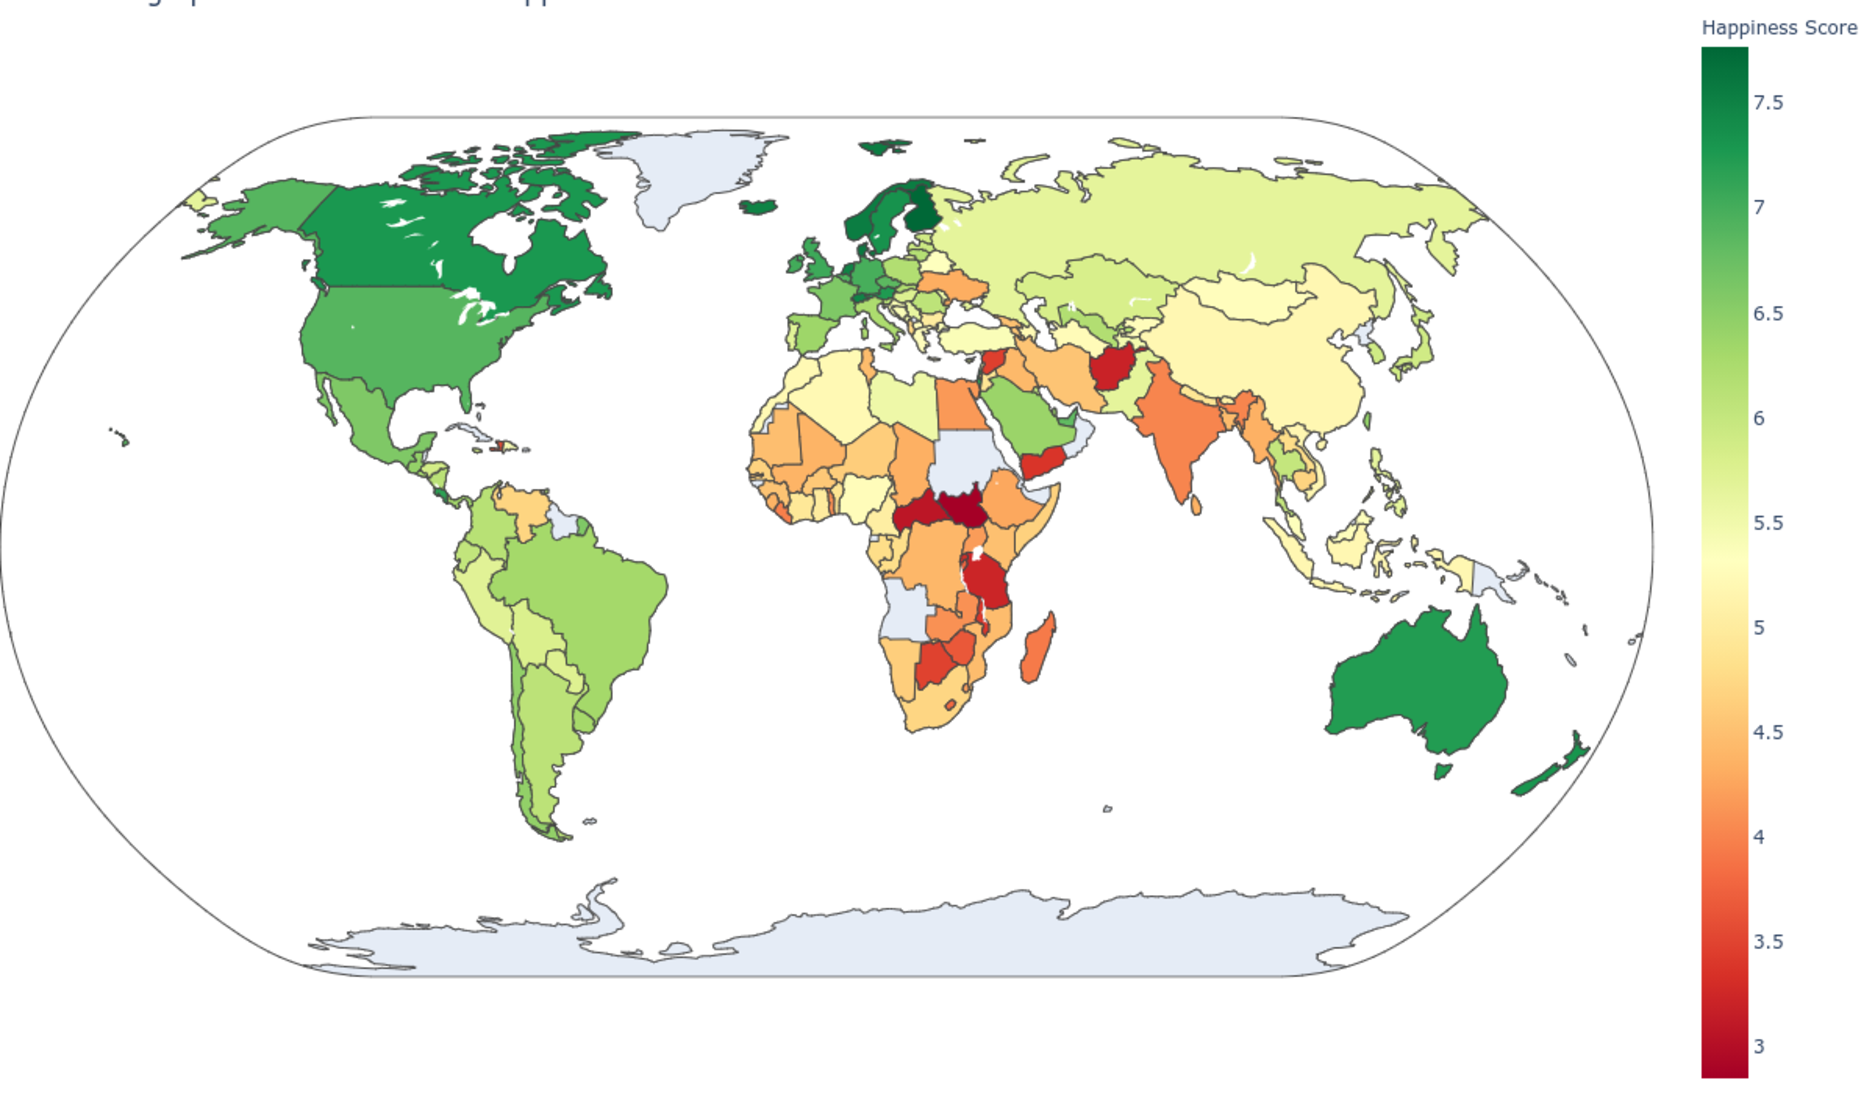
\includegraphics[height=.75\textheight]{score-worldmap.pdf}
  		\end{center}
	\end{frame}
	
	\begin{frame}{Introdução}
		\begin{center}
    	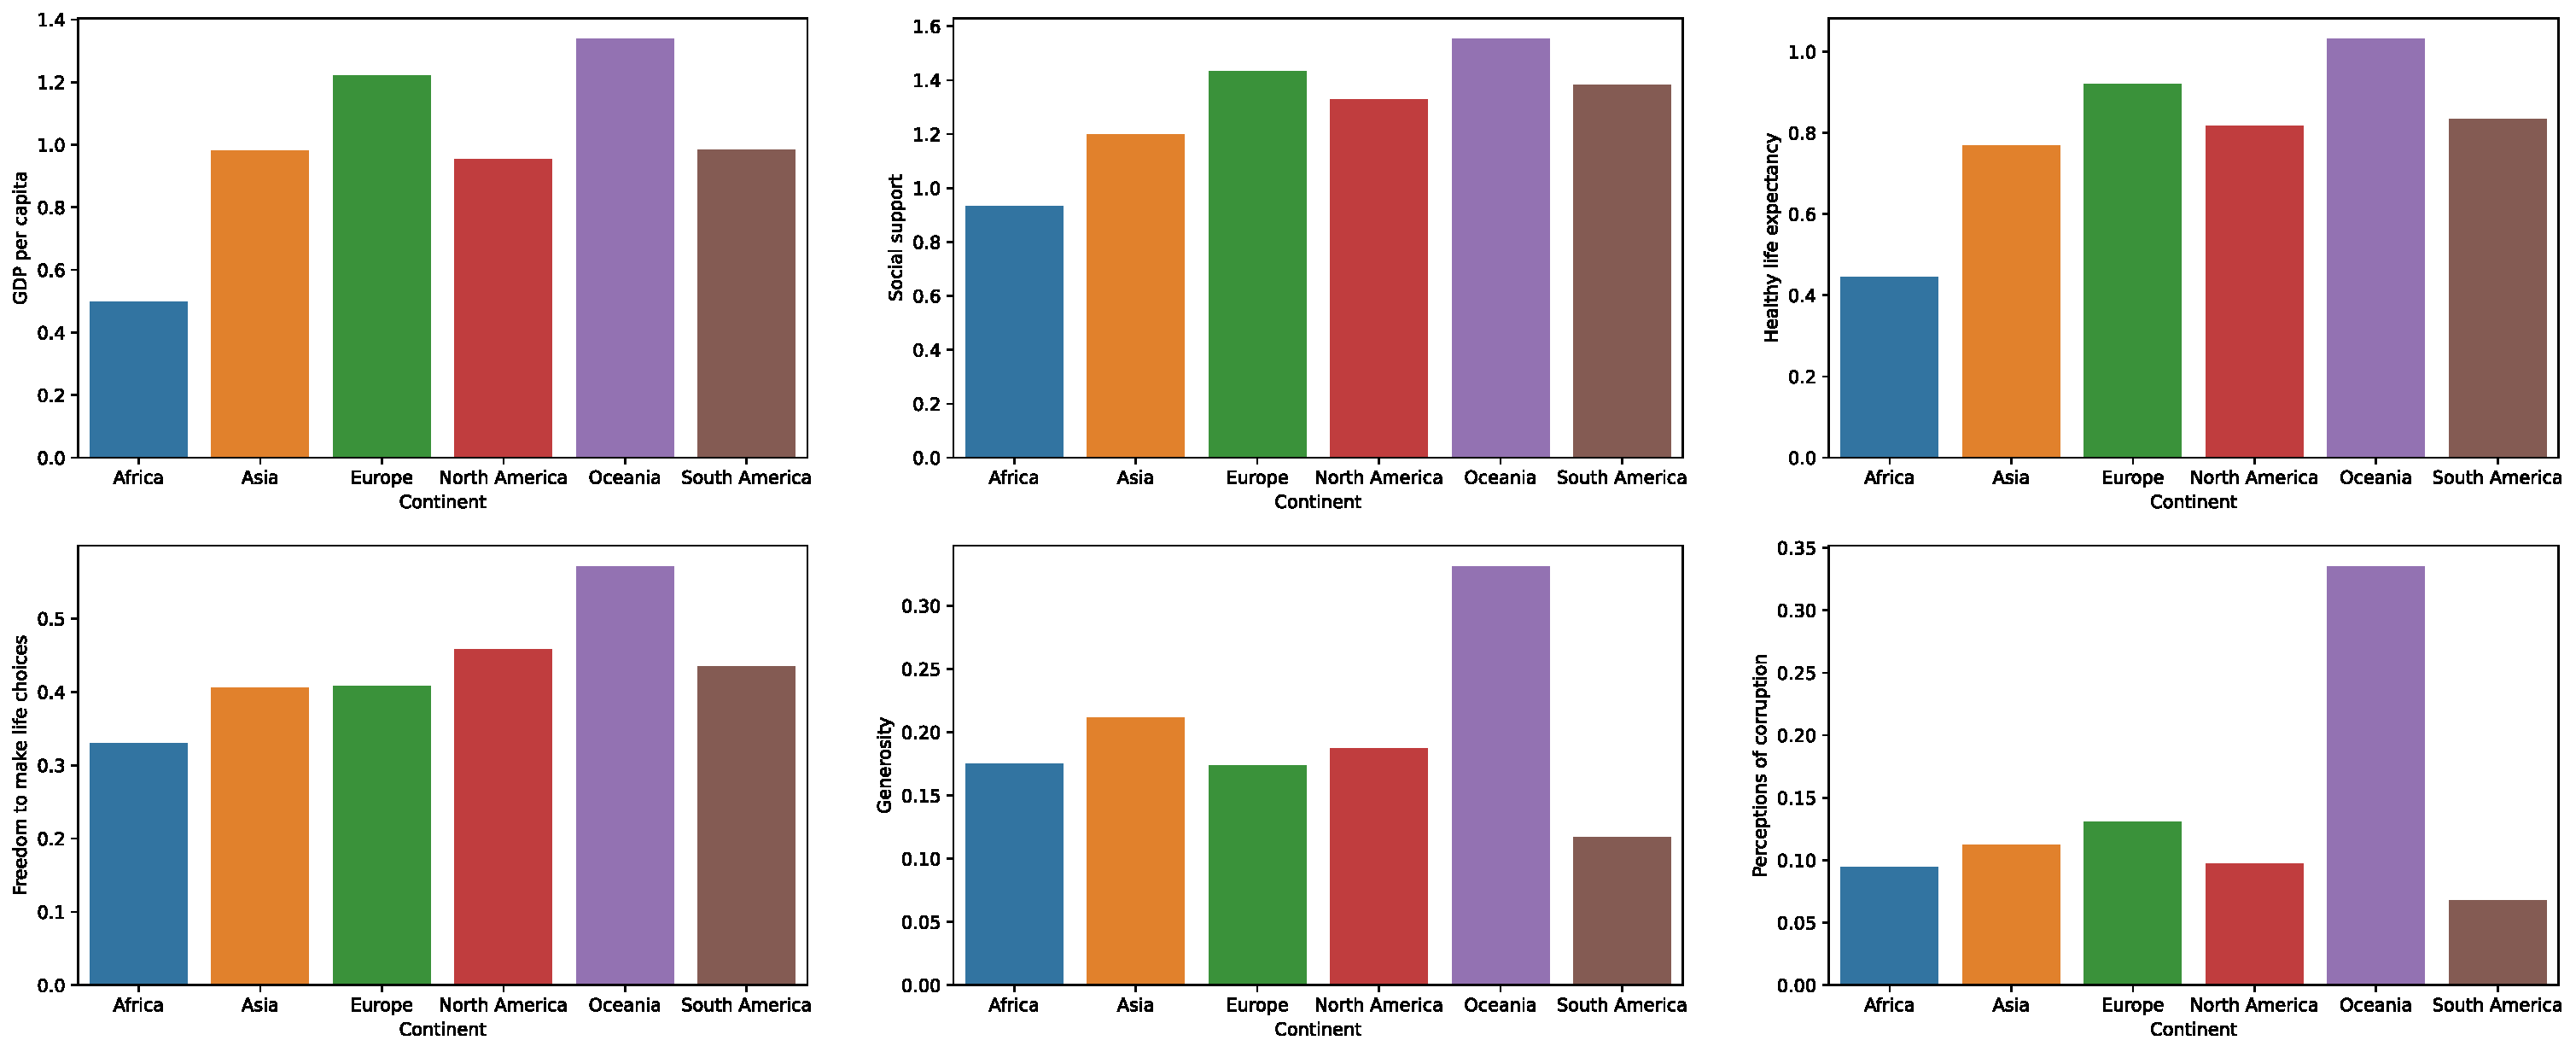
\includegraphics[height=.55\textheight]{variables-continents.pdf}
  		\end{center}
	\end{frame}
	
	\subsection{Análise Univariada}
	
	\begin{frame}{Análise Univariada}
        \begin{table}[ht]
        \centering
        \scalebox{0.7}{%
        \begin{tabular}{|l|c|c|c|c|c|c|c|}
        \hline
        \textit{\textbf{}} & \textit{\textbf{Score}} & \textit{\textbf{\begin{tabular}[c]{@{}c@{}}GDP\\ per\\ Capita\end{tabular}}} & \textit{\textbf{\begin{tabular}[c]{@{}c@{}}Social\\ support\end{tabular}}} & \textit{\textbf{\begin{tabular}[c]{@{}c@{}}Healthy\\ life\\ expectancy\end{tabular}}} & \textit{\textbf{\begin{tabular}[c]{@{}c@{}}Freedom\\ to make\\ life\\ choices\end{tabular}}} & \textit{\textbf{Generosity}} & \textit{\textbf{\begin{tabular}[c]{@{}c@{}}Perceptions\\ of\\ corruption\end{tabular}}} \\ \hline
        count & 156 & 156 & 156 & 156 & 156 & 156 & 156 \\ \hline
        mean & 5.407 & 0.905 & 1.208 & 0.725 & 0.392 & 0.184 & 0.110 \\ \hline
        std & 1.113 & 0.398 & 0.299 & 0.242 & 0.143 & 0.095 & 0.094 \\ \hline
        min & 2.853 & 0.000 & 0.000 & 0.000 & 0.000 & 0.000 & 0.000 \\ \hline
        25\% & 4.544 & 0.602 & 1.055 & 0.547 & 0.308 & 0.108 & 0.047 \\ \hline
        50\% & 5.379 & 0.960 & 1.271 & 0.789 & 0.417 & 0.177 & 0.085 \\ \hline
        75\% & 6.184 & 1.232 & 1.452 & 0.881 & 0.507 & 0.248 & 0.141 \\ \hline
        max & 7.769 & 1.684 & 1.624 & 1.141 & 0.631 & 0.566 & 0.453 \\ \hline
        IQR & 1.640 & 0.629 & 0.396 & 0.334 & 0.199 & 0.139 & 0.094 \\ \hline
        skew & 0.011 & -0.385 & -1.134 & -0.613 & -0.685 & 0.745 & 1.650 \\ \hline
        mad & 0.916 & 0.332 & 0.236 & 0.199 & 0.116 & 0.075 & 0.069 \\ \hline
        kurt & -0.608 & -0.769 & 1.229 & -0.302 & -0.068 & 1.173 & 2.416 \\ \hline
        \end{tabular}}
        \end{table}
	\end{frame}
	
	\begin{frame}{Análise Univariada}
		
	A retirar do sumário:
	
	\begin{itemize}
	    \item A média do \textit{Score} está próximo do meio da escala e o valor máximo é de 7.77 e
mínimo de 2.85;
        \item Metade dos países representados têm um \textit{Score} compreendido entre 4.5 e 6.2;
        \item Alguns países não têm dados relativos aos factores em causa, pois temos mínimos
de 0;
        \item As respectivas médias e medianas andam próximas, de onde concluímos que a distribuição dos valores será aproximadamente centrada.
        \item Dado o \textit{skewness}, nenhuma variável totalmente simétrica quanto à sua distribuição;
        \item Considerando \textit{Kurtosis}, probabilidade elevada de \textit{outliers} em \textit{Perceptions of corruption}.
	\end{itemize}
		
	\end{frame}
	
	\begin{frame}{Análise Univariada}
	    \begin{center}
    	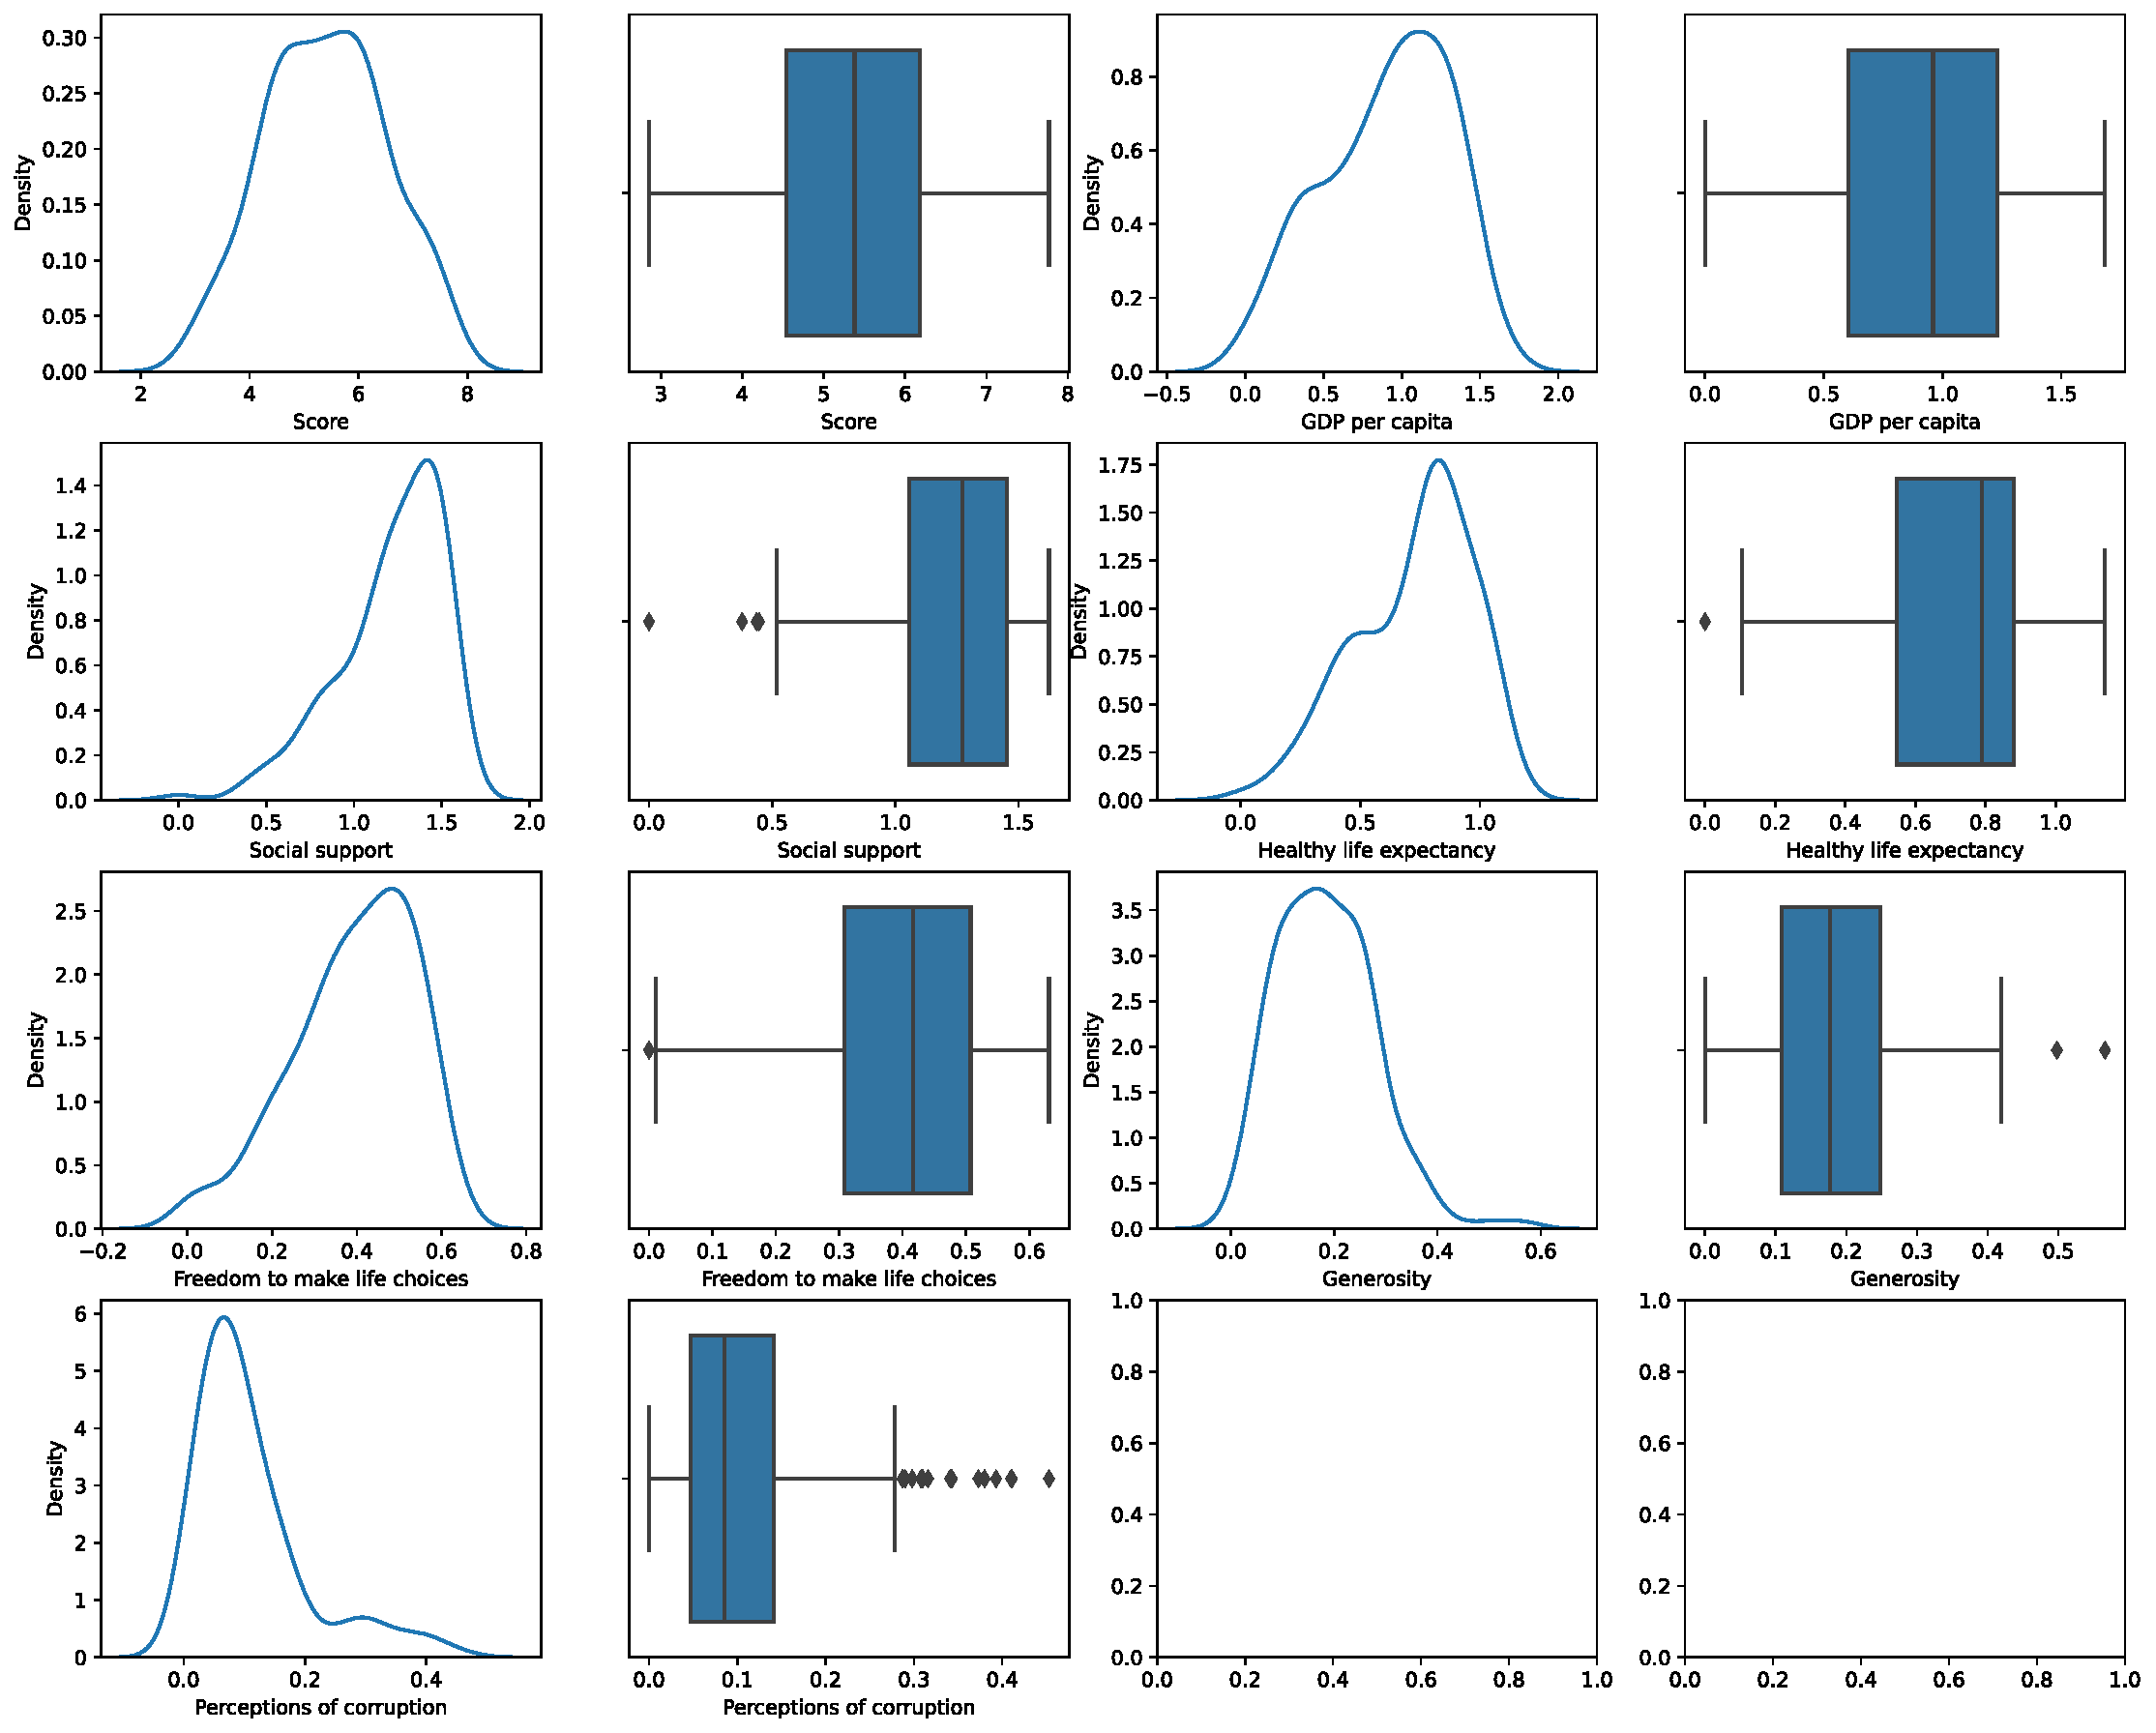
\includegraphics[height=.75\textheight]{boxplots3.pdf}
  		\end{center}
	\end{frame}
	
	
	\subsection{Análise Bivariada}
	
	\begin{frame}{Análise Bivariada}
	    \begin{center}
    	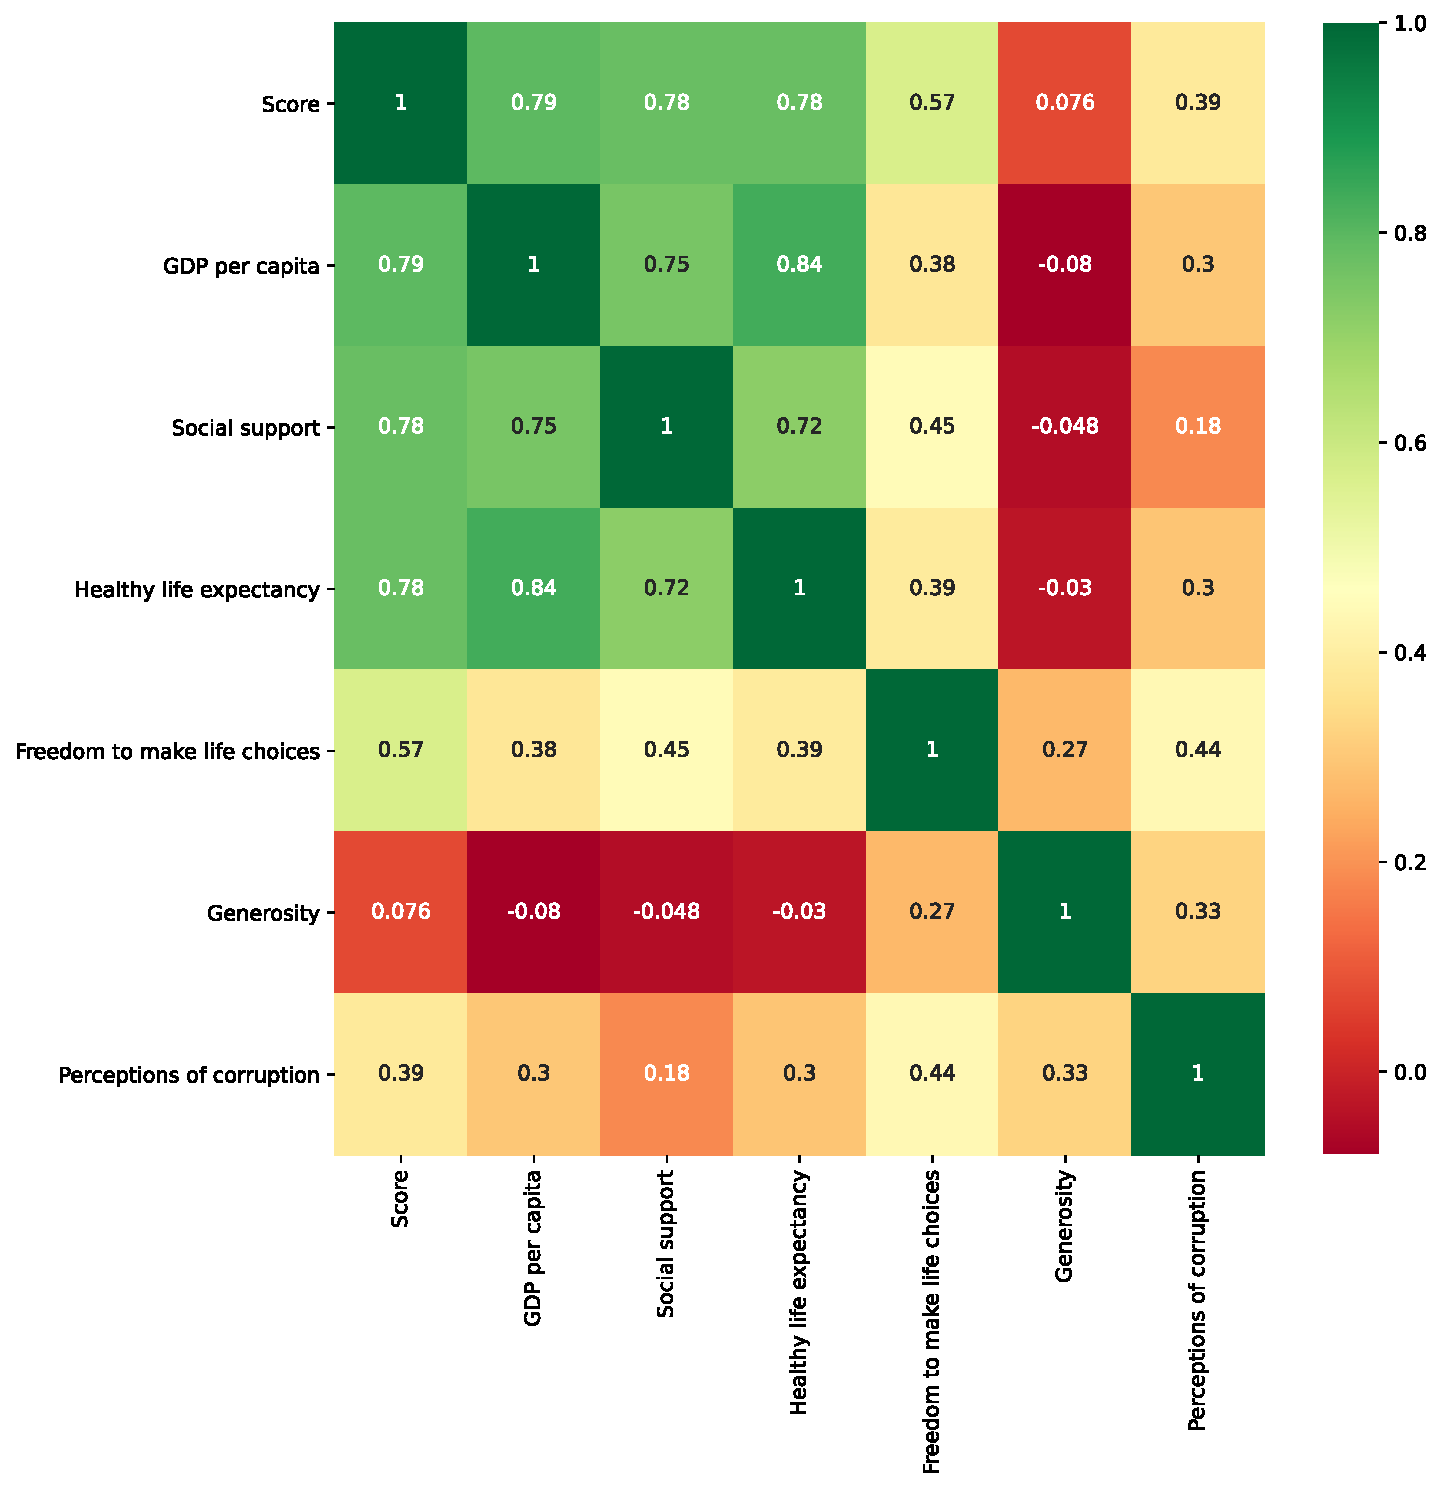
\includegraphics[height=.85\textheight]{corrmap.pdf}
  		\end{center}
	\end{frame}
	
	\begin{frame}{Análise Bivariada}
	A retirar da análise:
	    \begin{itemize}
	        \item \textit{Score} com correlação positiva com todas as outras variáveis (praticamente nula com \textit{Generosity});
	        \item Correlações positivas esperadas:
	            \begin{itemize}
	                \item \textit{GDP per capita} e \textit{Social support};
	                \item \textit{GDP per capita} e \textit{Healthy life expectancy};
	                \item \textit{Social support} e \textit{Healthy life expectancy};
	            \end{itemize}
	    \end{itemize}
	\end{frame}
	
	\section{\textit{Factor Analysis}}
	\subsection{Normalização}
	\subsection{Teste de adequação}
	\begin{frame} {Testes de adequação}
	
	Foram realizados diversos testes a fim de aferir a adequação dos dados à FA:
	
	\begin{itemize}
	\item Teste de Bartlett, tendo com hipótese nula a matriz de correlações tratar-se de uma matriz de identidade, Obteve-se um valor de chi-quadrado de aproximadamente 656 e o nível de significância obtido foi de 0.0, indicando a rejeição da hipótese nula;
	\item KMO, tendo-se obtido o valor de 0.84 (forte adequação);
	
	\item Measure of Sampling Adequacy (MSA), tendo sido os valores obtidos superiores a 0.5 para todas as varíaveis. 
	\end{itemize}
	
	\end{frame}
	\subsection{PCA}
		\begin{frame}{PCA}
		\begin{table}[h]
        \centering
        \scalebox{0.7}{%
        \begin{tabular}{c|c|c|c|}
        \cline{2-4}
         & \textbf{Eigenvalue} & \textbf{\begin{tabular}[c]{@{}c@{}}Fracção de Variância\\ Explicada (\%)\end{tabular}} & \textbf{Fracção Acumulada (\%)} \\ \hline
        \multicolumn{1}{|c|}{1} & 3.837141 & 54.46 & 54.46 \\ \hline
        \multicolumn{1}{|c|}{2} & 1.436346 & 20.39 & 74.85 \\ \hline
        \multicolumn{1}{|c|}{3} & 0.616839 & 8.76 & 83.61 \\ \hline
        \multicolumn{1}{|c|}{4} & 0.559896 & 7.95 & 91.56 \\ \hline
        \multicolumn{1}{|c|}{5} & 0.263794 & 3.74 & 95.30 \\ \hline
        \multicolumn{1}{|c|}{6} & 0.173418 & 2.46 & 97.76 \\ \hline
        \multicolumn{1}{|c|}{7} & 0.157726 & 2.24 & 100.00 \\ \hline
        \end{tabular}}
        \end{table}
	
	
	\end{frame}
	
	
	\begin{frame}{PCA}
	
		\begin{center}
    	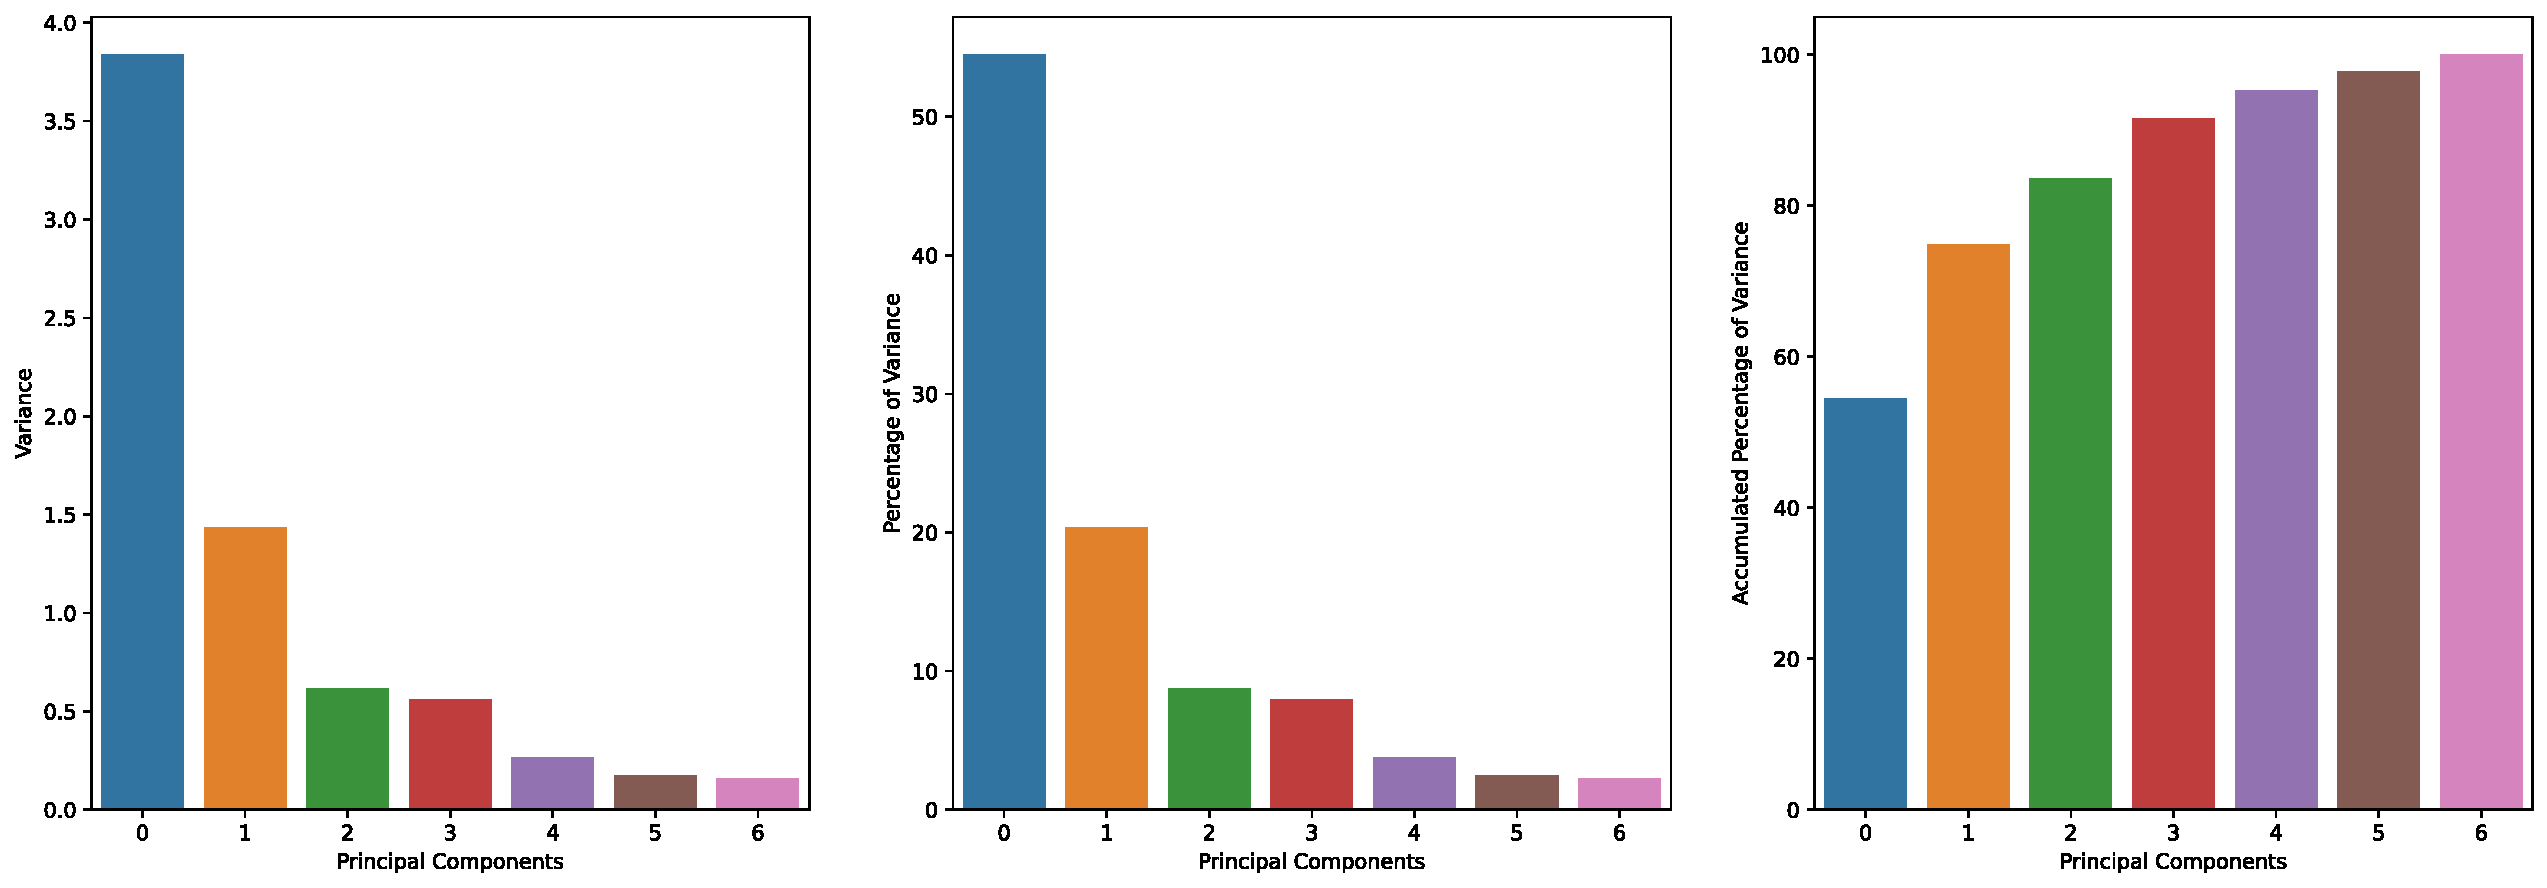
\includegraphics[height=.50\textheight]{PrincipalComponents.pdf}
  		\end{center}
	
	
	\end{frame}
	\begin{frame}{PCA - Seleção nº componentes}
	
	Seguindo o critério de Kaiser (\textit{eigenvalue} > 1) mantiveram-se 2 componentes, explicando, assim, aproximadamente 75\% da variância. 
	
	
	
	
	\end{frame}
	
	
	\begin{frame}{Correlações componentes e varíaveis}
		\begin{table}[h]
        \centering
        \scalebox{0.7}{%
        \begin{tabular}{|l|c|c|}
        \hline
        \textit{\textbf{Features}} & \textbf{PC1} & \textbf{PC2} \\ \hline
        \textit{Score} & \cellcolor[HTML]{FFCC67}-0.475861 & -0.028371 \\ \hline
        \textit{GDP} & \cellcolor[HTML]{FFCC67}-0.454825 & -0.213377 \\ \hline
        \textit{Healthy life exp} & \cellcolor[HTML]{FFCC67}-0.436582 & -0.207148 \\ \hline
        \textit{Social support} & \cellcolor[HTML]{FFCC67}-0.450150 & -0.177856 \\ \hline
        \textit{Freedom} & -0.332201 & 0.362130 \\ \hline
        \textit{Generosity} & -0.048232 & \cellcolor[HTML]{FFCC67}0.693809 \\ \hline
        \textit{Corruption} & -0.246511 & \cellcolor[HTML]{FFCC67}0.516346 \\ \hline
        \end{tabular}}
        \end{table}
	
	\end{frame}
	
	\begin{frame}{Círculo de correlações}
	
		\begin{center}
    	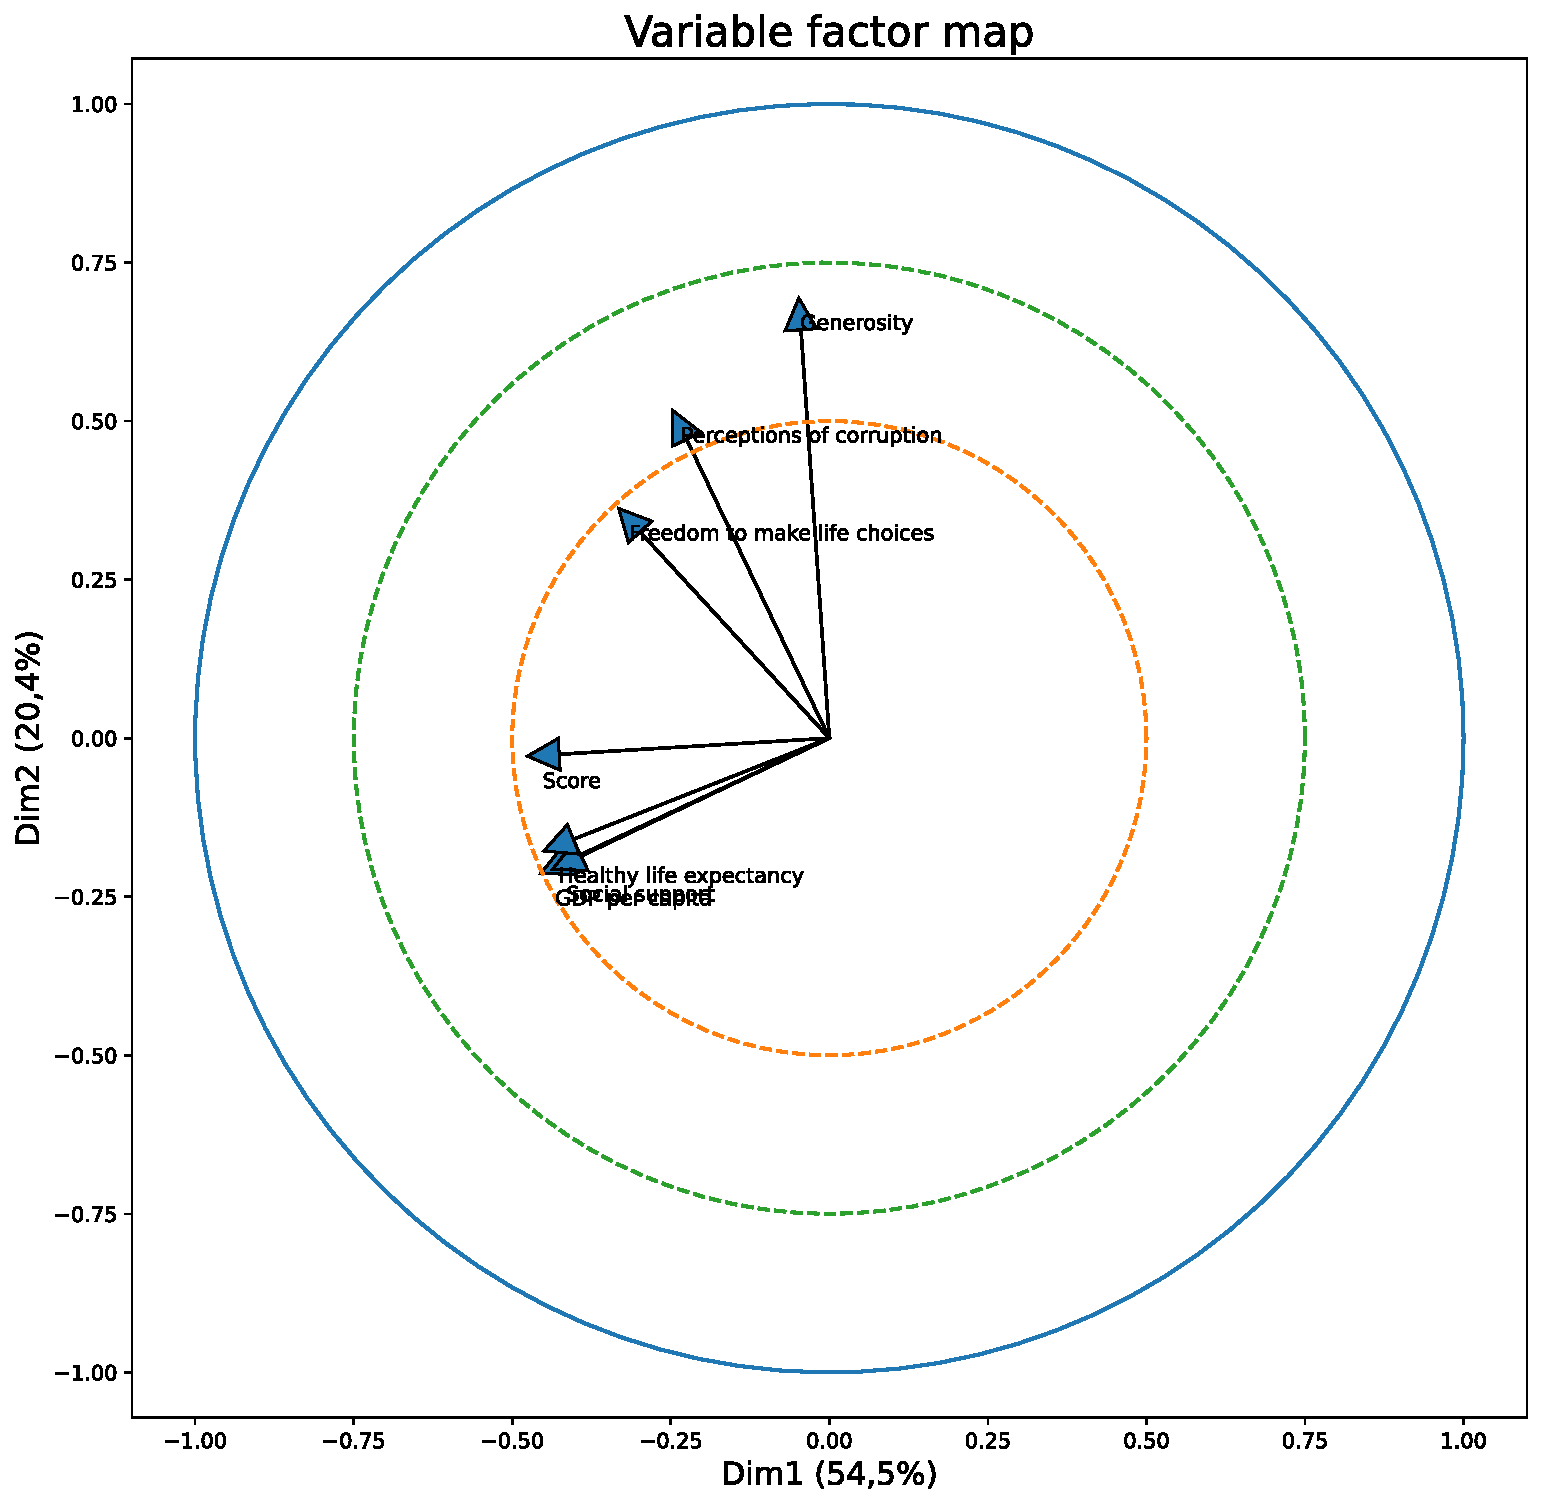
\includegraphics[height=.65\textheight]{VariableFactorMap1.pdf}
  		\end{center}
	
	\end{frame}
	
	\begin{frame}{Factor Analysis}
	    Foi realizada Factor Analysis com dois factores, tendo-se utilizado rotação \textit{varimax}.
	    
		\begin{table}[h]
        \centering
        \scalebox{0.7}{%
        \begin{tabular}{l|c|c|c|c|}
        \cline{2-5}
         & \textit{\textbf{Factor 1}} & \textit{\textbf{Factor 2}} & \textit{\textbf{Communalities}} & \textit{\textbf{Variância específica}} \\ \hline
        \multicolumn{1}{|l|}{\textit{\textbf{Score}}} & 0.886962 & 0.278875 & 0.864474 & 0.14 \\ \hline
        \multicolumn{1}{|l|}{\textit{\textbf{GDP}}} & 0.922187 & 0.056855 & 0.853661 & 0.15 \\ \hline
        \multicolumn{1}{|l|}{\textit{\textbf{Healthy life exp.}}} & 0.886130 & 0.051952 & 0.787925 & 0.21 \\ \hline
        \multicolumn{1}{|l|}{\textit{\textbf{Social support}}} & 0.899390 & 0.093791 & 0.817701 & 0.18 \\ \hline
        \multicolumn{1}{|l|}{\textit{\textbf{Freedom}}} & 0.466562 & 0.624670 & 0.607894 & 0.39 \\ \hline
        \multicolumn{1}{|l|}{\textit{\textbf{Generosity}}} & -0.188509 & 0.812598 & 0.695852 & 0.30 \\ \hline
        \multicolumn{1}{|l|}{\textit{\textbf{Corruption}}} & 0.247258 & 0.742319 & 0.612174 & 0.39 \\ \hline
        \end{tabular}}
        \end{table}
	
	
	\end{frame}
	
	
	\begin{frame}{Projeção dos Indíviduos}
	   
		\begin{center}
    	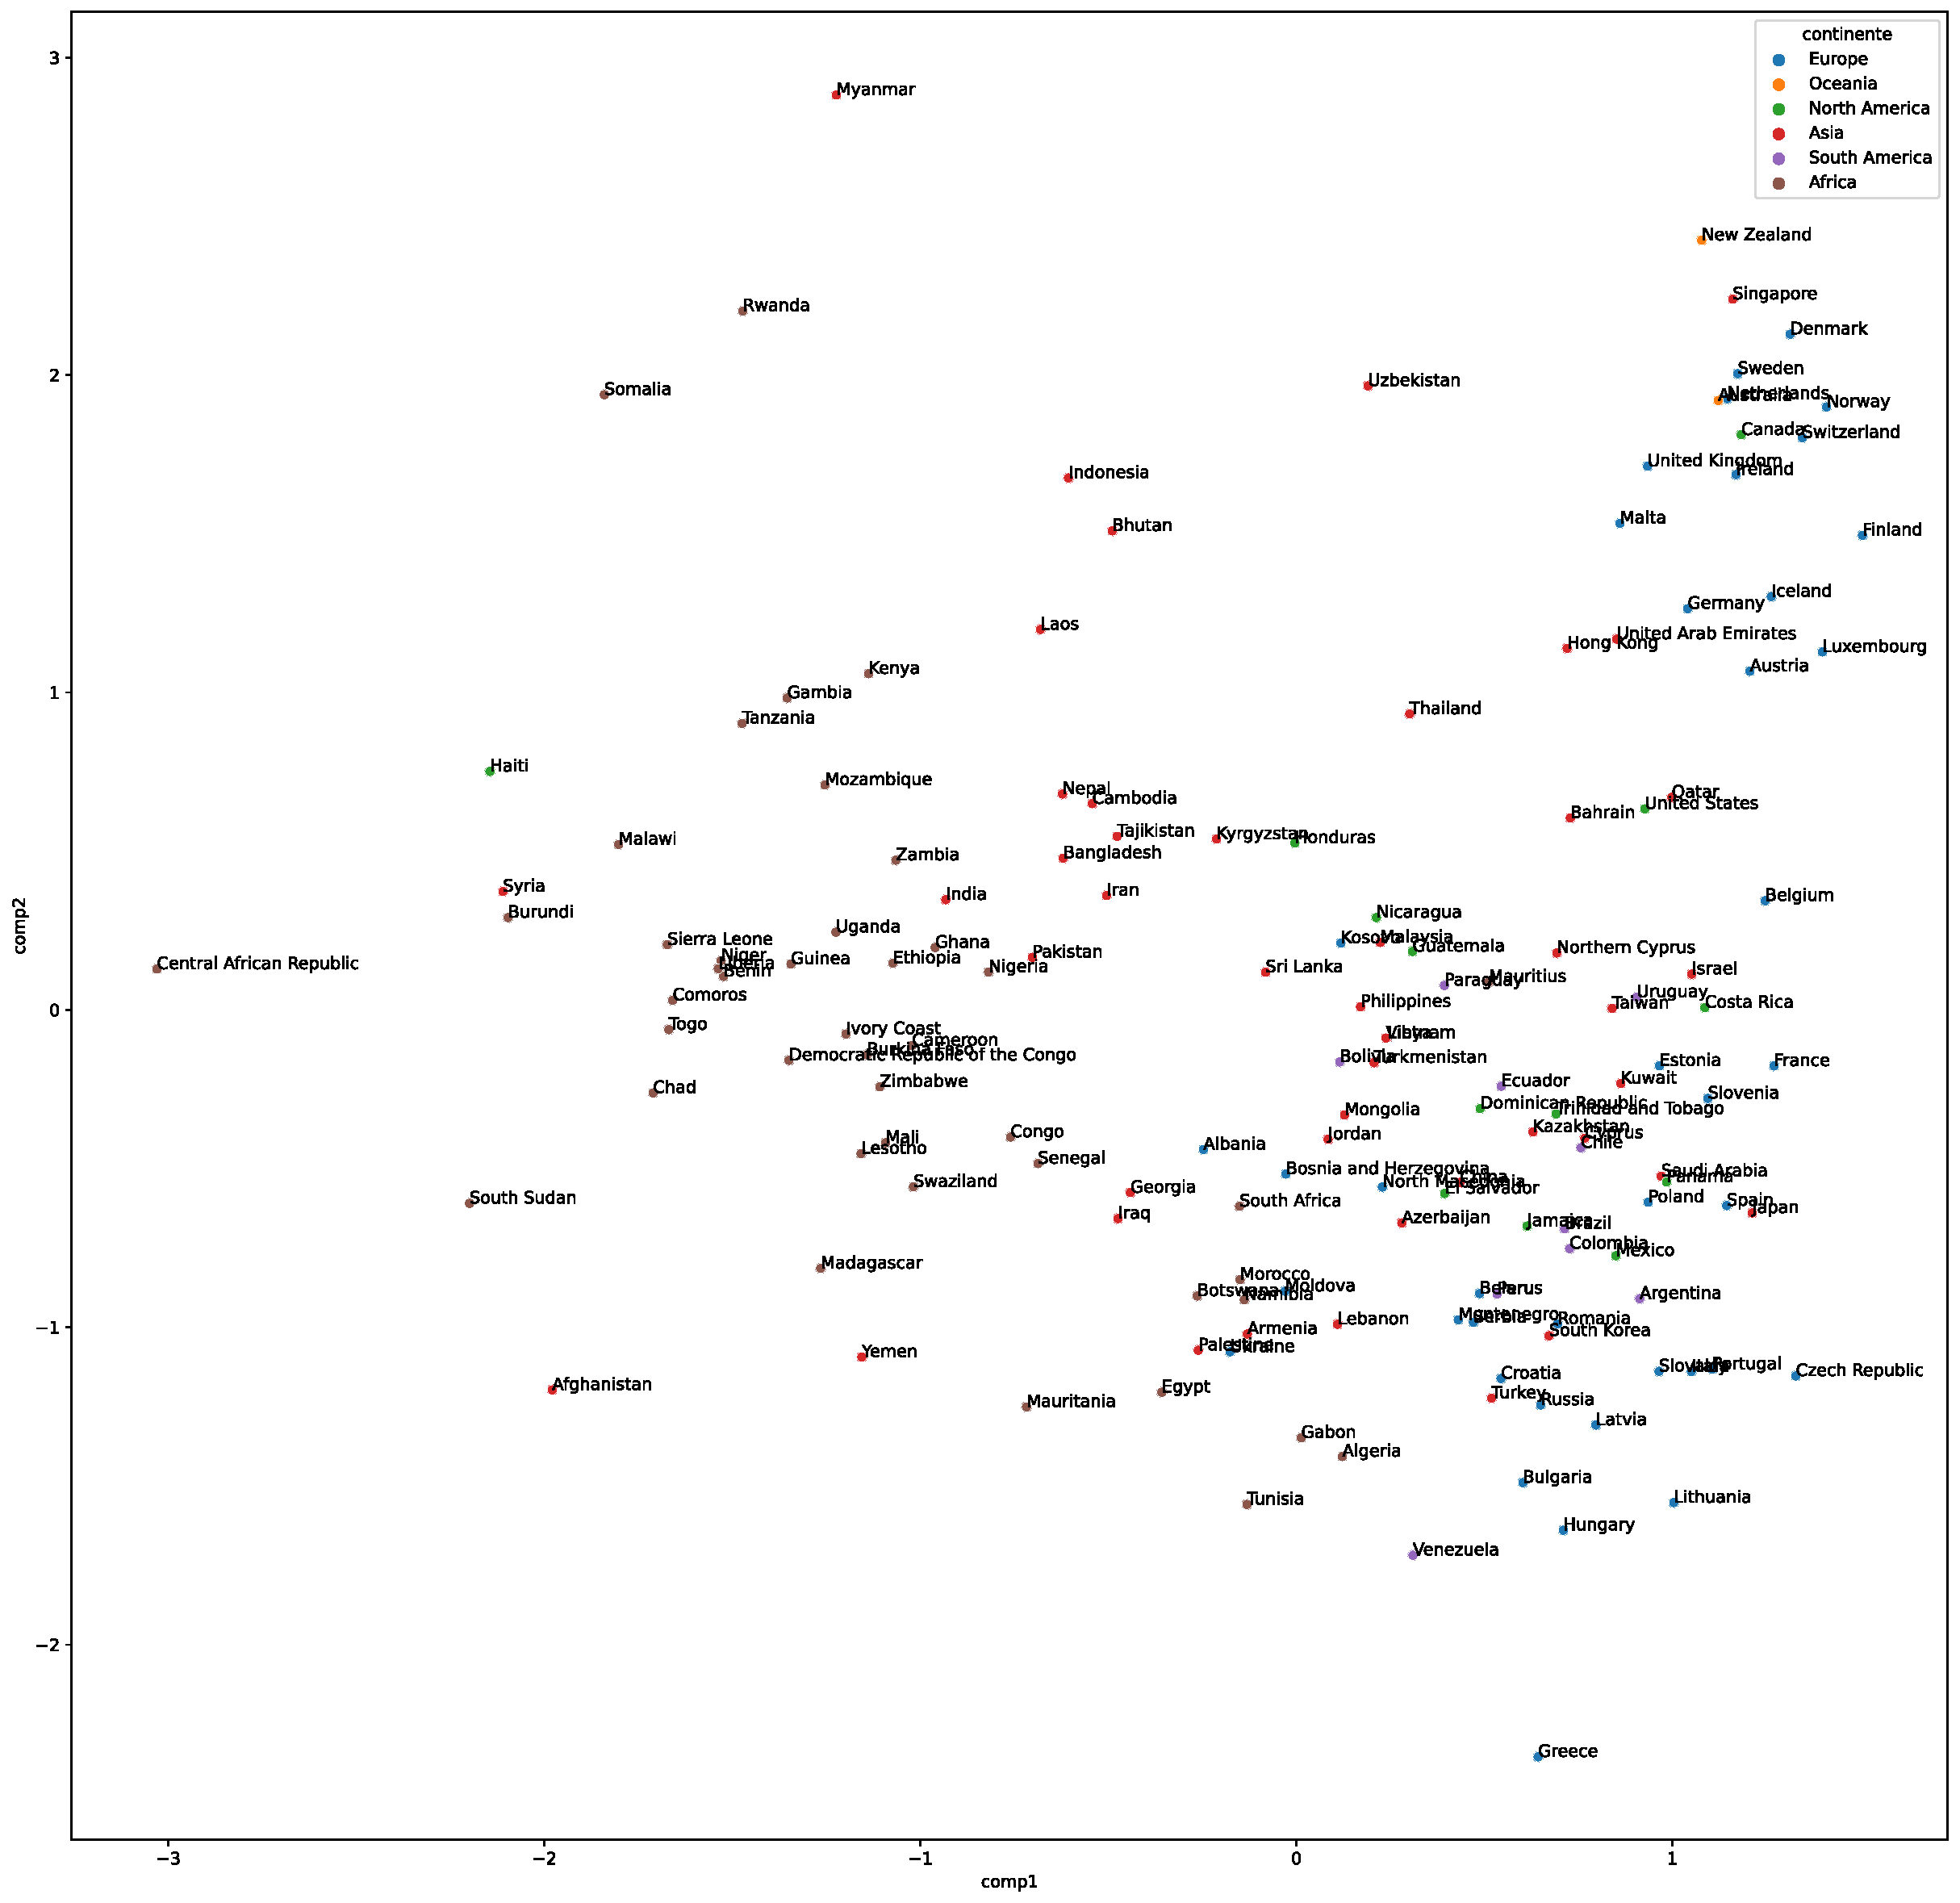
\includegraphics[height=.90\textheight]{IndividualsMap.pdf}
  		\end{center}
	
	\end{frame}
	
	\section{Conclusão}
	\begin{frame}{Conclusão}
	Com a realização deste trabalho foi possível:
	    \begin{itemize}
	        \item Realizar análise univariada e bivariada dos dados;
	        
	        \item Representar o dataset recorrendo a apenas 2 componentes, explicando 75\% da variância;
	        
	    \end{itemize}
	\end{frame}
	

	
	
%		\begin{center}
%    	\includegraphics[height=.65\textheight]{images/santa.png}
%  		\end{center}
	
	

	

\end{document}